
\chapter{Background}
In this chapter, I discuss the overall project of which the 408 nm 5 GHz detuned laser system is a part. I will give a detailed summary of the preparation the atoms undergo before they are manipulated by the laser system whose construction is the main topic of this thesis. I will also discuss the ion interferometer project vis-\`a-vis other physics experiments. 

\section{Ion Interferometer Basic Overview}
The central feature of any interferometer is that there is some travelling wave that is split and sent along two distinct paths. At some later point, the waves from the two paths are recombined. The output of the interferometer depends on the relative phase acquired by the wave as it travels along the two distinct paths of the interferometer.
The goal of the ion interferometer project is to create an interferometer that uses atomic wavefunction of a beam of travelling Strontium ions to achieve interference.
In other words, we hope to split and recombine the atomic wavefunction of Strontium ions in such a way that the atomic wavefunction is nonzero along two distinct paths through space. 
The output of the interferometer gives information about the relative phase shift acquired by the atoms as they travel along each of the arms of the interferometer. 

The $^{87}$Sr$^+$ ion interferometer uses a Mach-Zehnder configuration, which refers to the fact that the two paths along which the waves travel enclose a non-zero area. Fig.\ \ref{mach-zehnder-fig} illustrates an optical Mach-Zehnder interferometer and compares this with the matterwave Mach-Zehnder interferometer that we are trying to build.

\begin{figure}
\centerline{
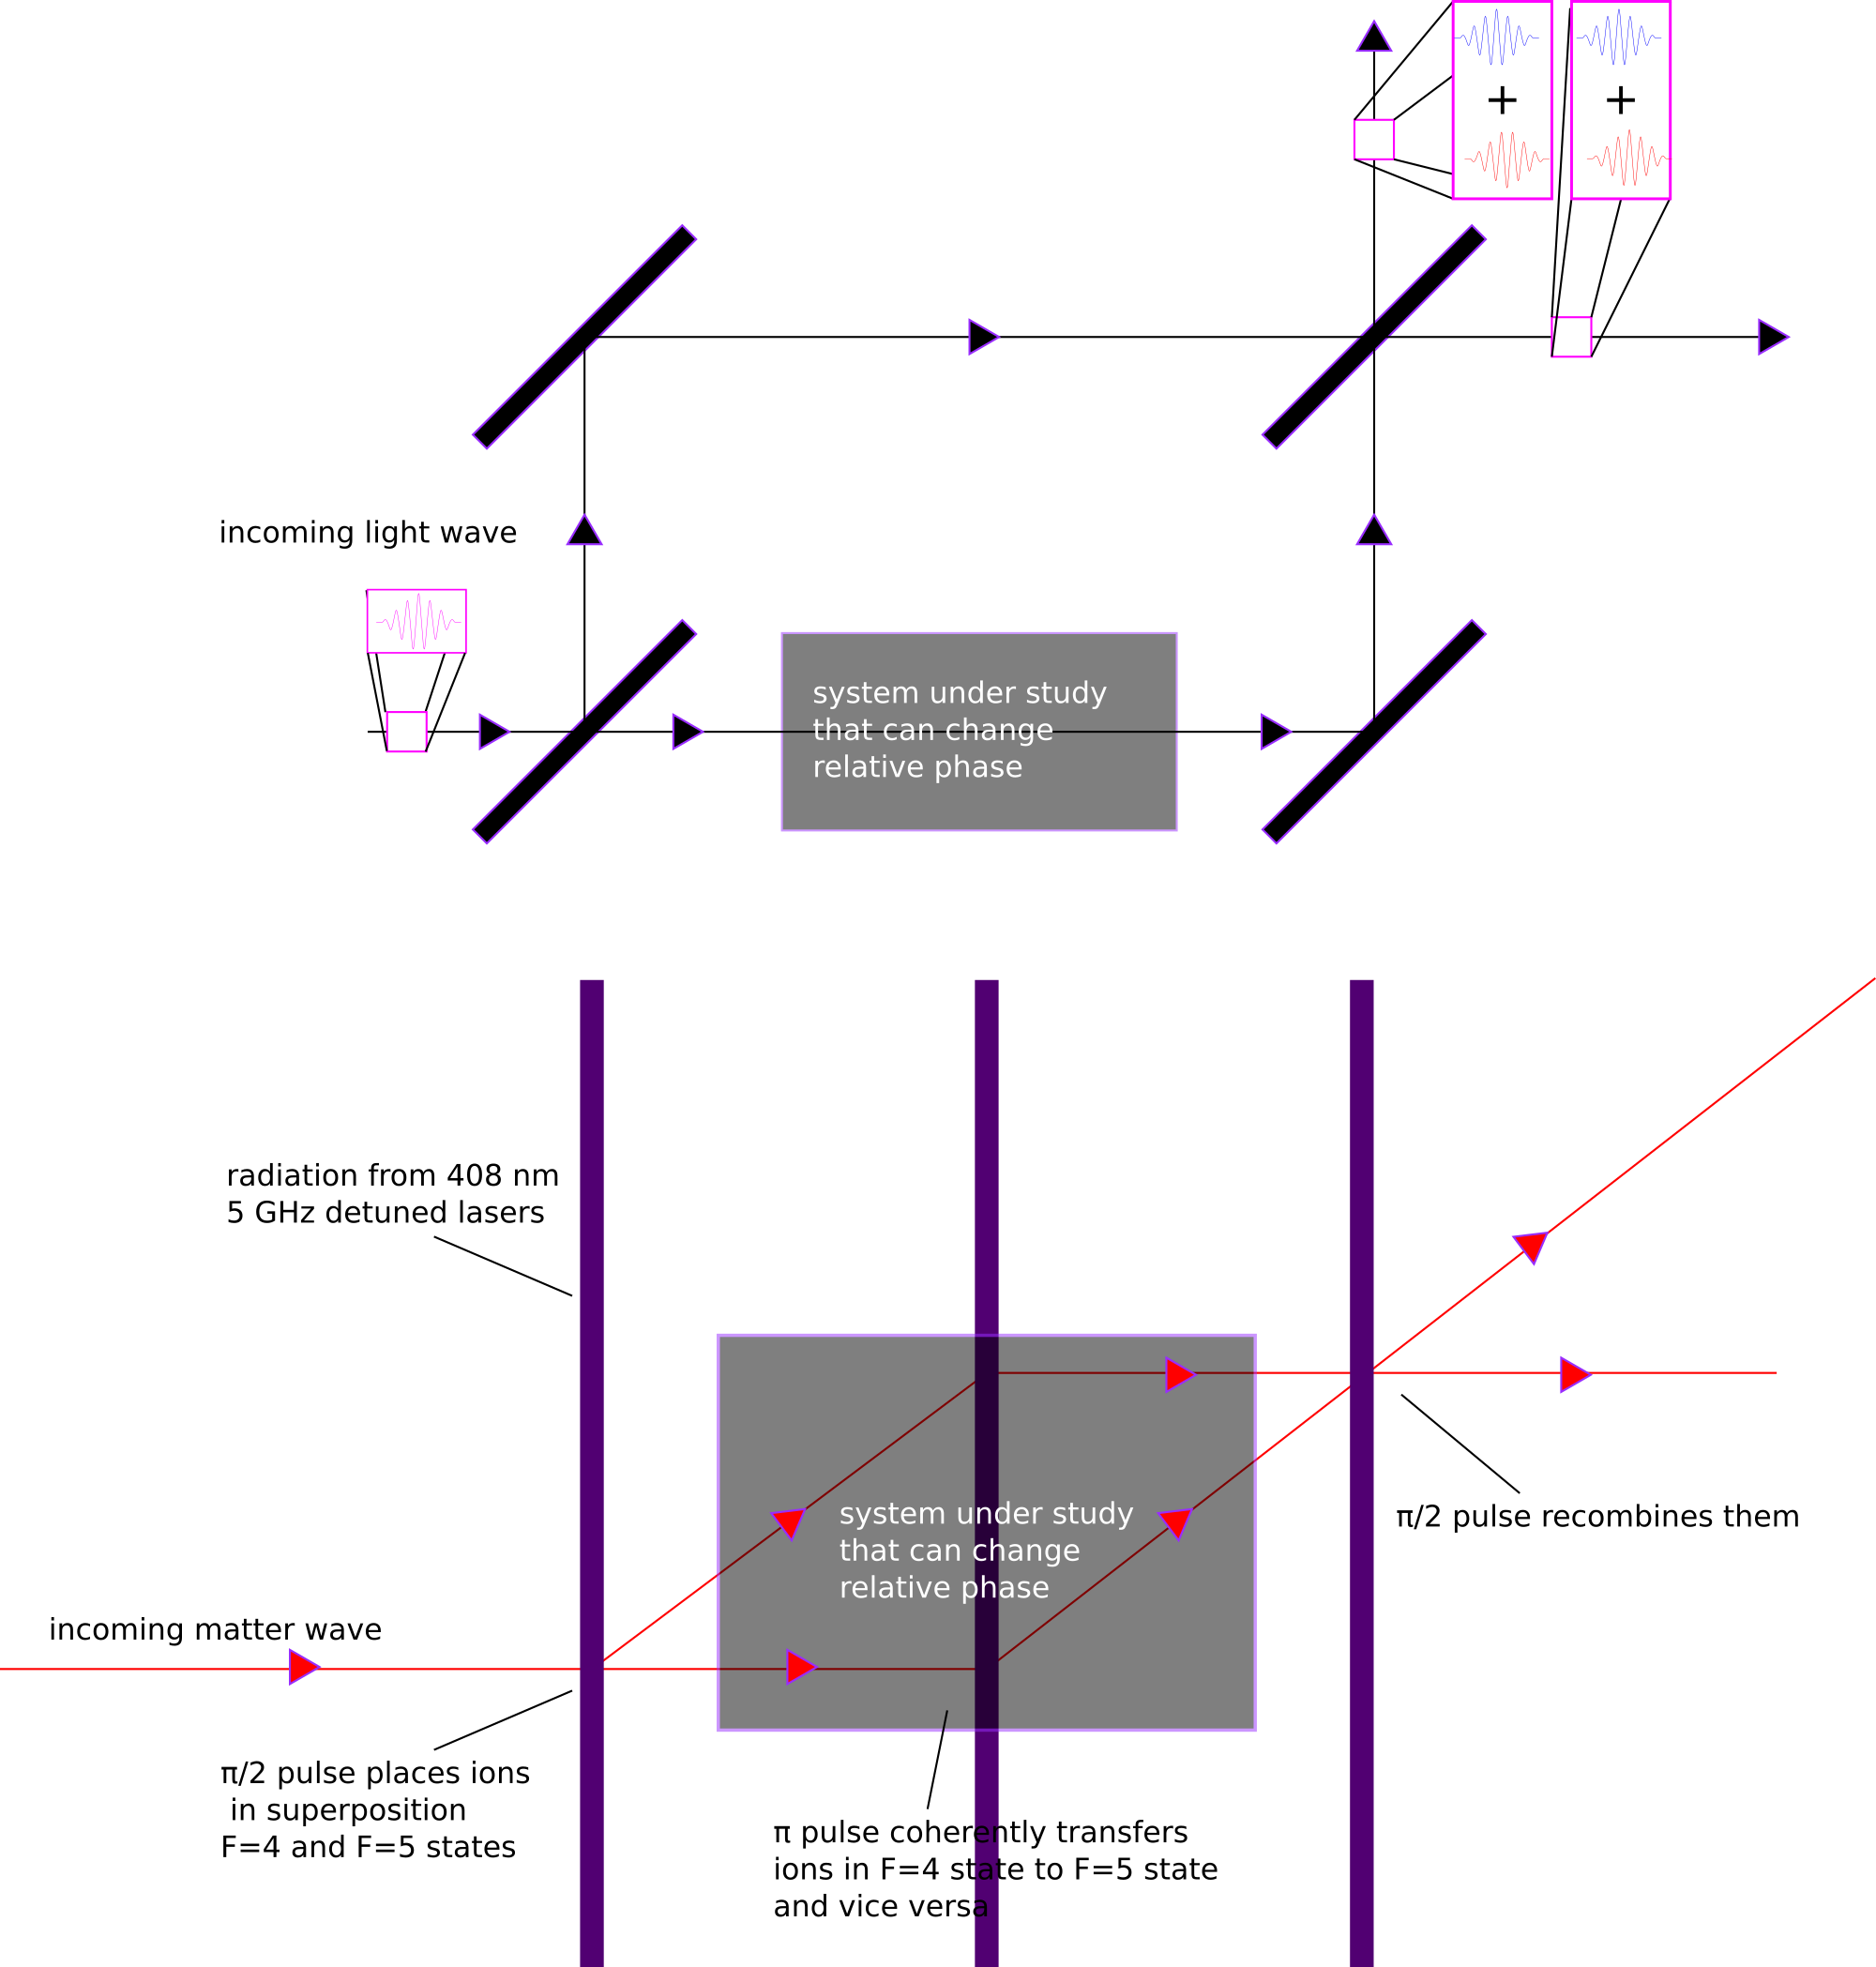
\includegraphics[width=0.95\textwidth]{mach-zehnder}}
\caption[Optical and Matterwave Mach-Zehnder interferometers]{\label{mach-zehnder-fig}A traditional realization of an optical Mach-Zehnder interferometer (top) juxtaposed with a sparse diagram of the ion interferometer (bottom). The optical Mach-Zehnder interferometer achieves interference of light waves and uses traditional glass optics to split and recombine the beams. The ion interferometer is designed to achieve interference of matter waves. The ion interferometer splits the atomic wavefunction of the Strontium ions using continuous wave lasers. These lasers manipulate the ions in a coherent way and place them in a superposition of states that correspond to taking one path or the other.}
\end{figure}

In order to accomplish ion interferometry, we must first acquire a suitable source of $^{87}$Sr$^+$ ions. There are three basic processes that must be accomplished with the Sr atoms in order to successfully operate the interferometer: 
\begin{itemize}
\item Generation of a low velocity beam of cold, neutral Strontium atoms   
\item Ionization of Strontium Atoms
\item Atom interferometry
\end{itemize} 
A schematic of the apparatus is depicted in Figure~\ref{fig:IonInterferometer}.

\begin{figure}
\centerline{
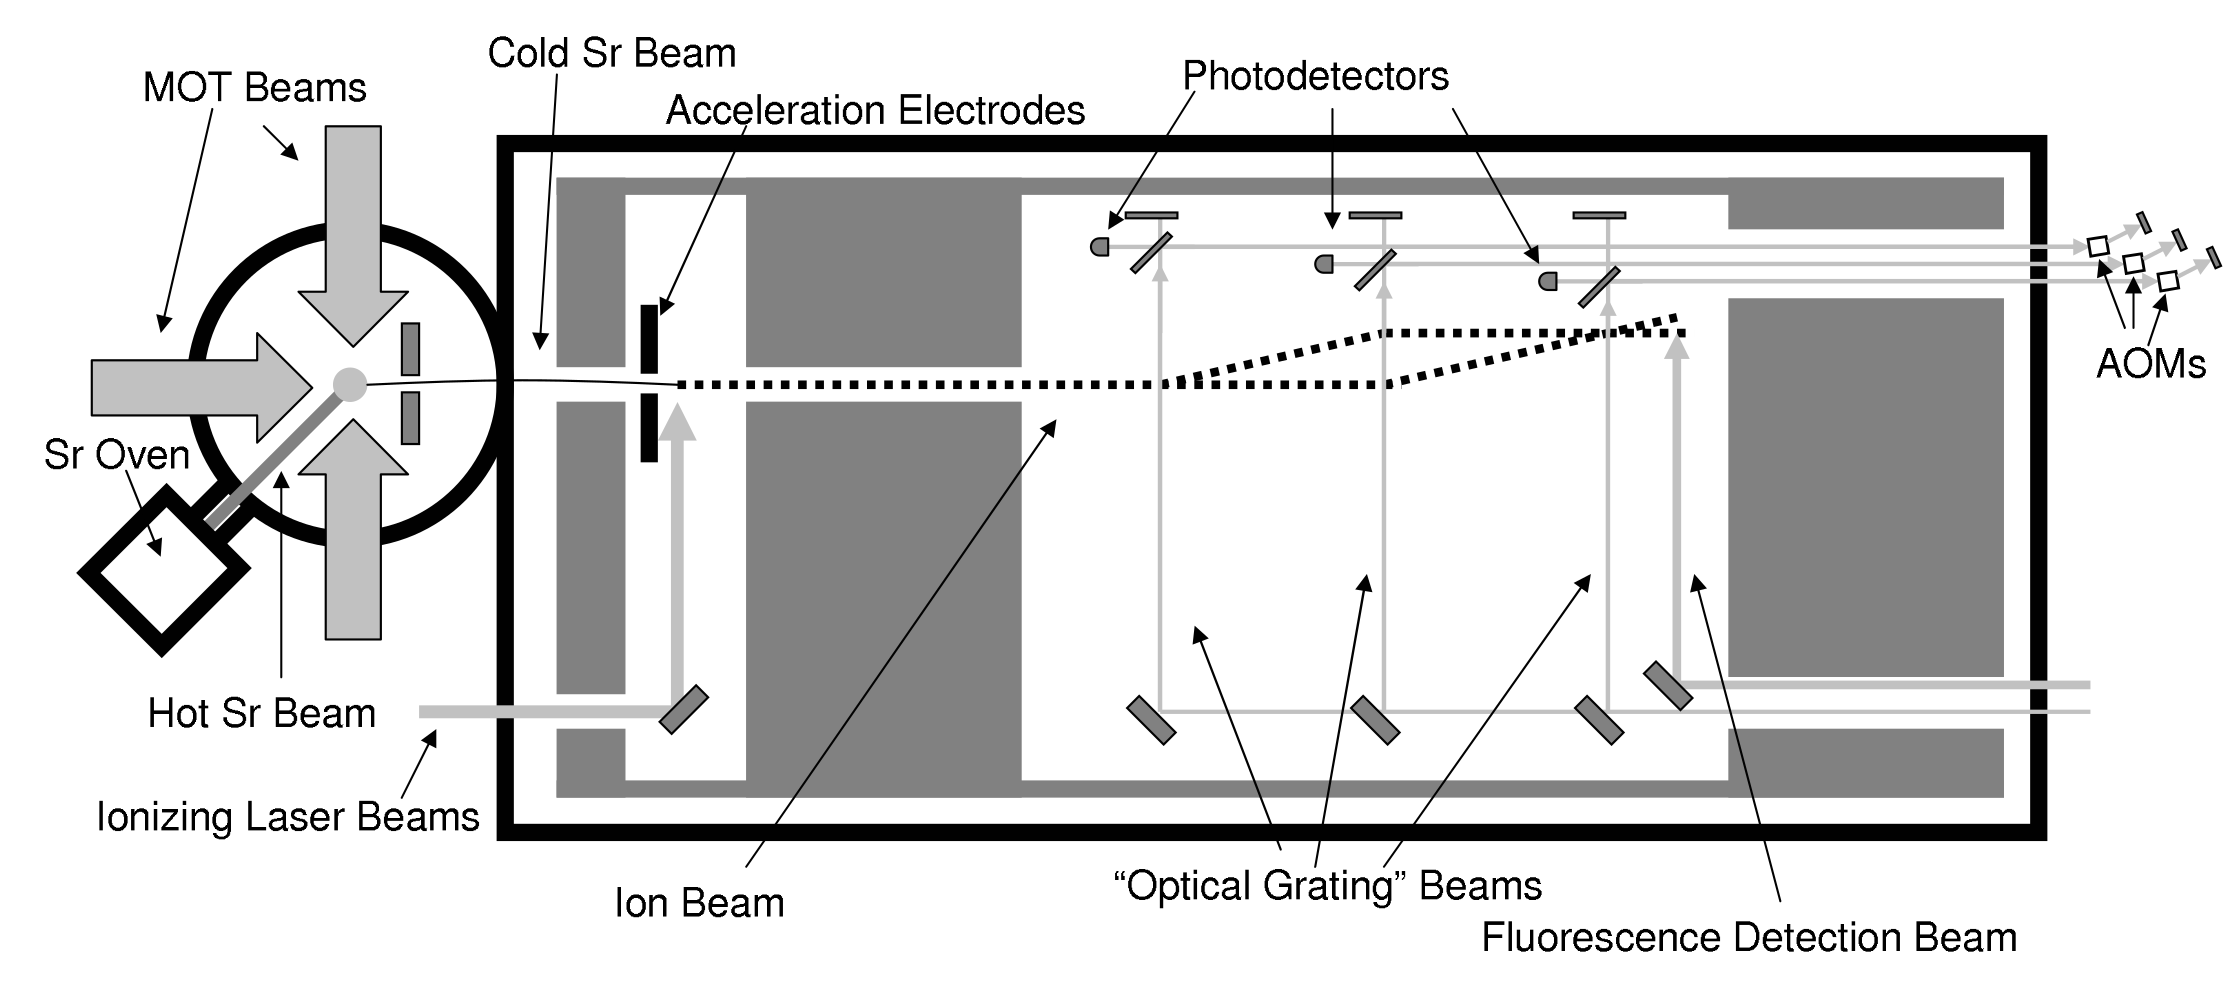
\includegraphics[totalheight=0.3\textheight]{interferometer_diagram}
}
\caption[Ion Interferometer]{\label{fig:IonInterferometer}
A schematic diagram of the $^{87}$Sr$^+$ ion interferometer. Neutral strontium atoms start out in the Sr Oven depicted on the left part of the diagram. The heated chunks of strontium release atoms into the vacuum chamber where some of them are cooled and trapped by the MOT beams. One of the mirrors used on the MOT beams has a hole in it, which allows some of the ions to escape. The MOT with a hole in it comprises the Low Velocity Intense Source (LVIS). Neutral atoms that emerge from the LVIS enter a larger vacuum chamber where they are ionized by a pair of lasers. After this, they are accelerated by an electric field into the part of the chamber where actual interferometry will take place. The ``Optical Grating'' Beams are generated by the 408 nm 5GHz detuned laser system that is the topic of this thesis.} 
\end{figure}

\section{Trapping of Neutral Strontium and Low Velocity Intense Source (LVIS)}

We created a Low Velocity Intense Source (``LVIS'' pronounced ``Elvis'') \cite{cjeDiss} that provides a cold beam of slow-moving, neutral Strontium atoms. The techniques we used were developed by the Cornell group at UC Boulder\cite{LVIS}. The LVIS consists of a Magneto-Optical Trap (MOT) where one of the mirrors has a small hole drilled in it\footnote{This hole was drilled in-house and the details of how we avoided damage and tests that verify the integrity of its optical surface can be found in Ref.\,\cite{cjeDiss}.}. This allows some of the atoms to escape the trap. These atoms have a relatively narrow distribution of velocities. %\footnote{Probably cite some other reference here--whoever invented/talked about the LVIS}

The MOT at the heart of the LVIS uses the standard techniques for cooling and trapping atoms, as described by Erickson\cite{cjeDiss}. It utilizes the 5s$^2$ $^1$S$_0$ to 5s5p $^1$P$_1$ transition in neutral $^{87}$Sr to cool and trap the atoms. It selectively traps only the $^{87}$Sr isotope of strontium. The trap consists of 6 red-detuned laser beams originating from the 460.8 nm laser system described in Ref.\,\cite{cjeDiss}. These point from each of six orthogonal directions towards the center of the MOT. The dominant cooling effect in the MOT is Doppler cooling. 
The trap also relies on the magnetic field produced by a pair of permanent rare-earth magnets. This magnetic field causes the atoms to experience a Zeeman shift whose magnitude depends on their location. This process effectively confines the coldest atoms to a small region. 

The MOT is loaded via a Sr oven. The Sr vapor that is produced by heating a sample of Sr passes through a small Zeeman slower in order to maximize the quantity of atoms inside the trap. 


%Incidentally, this cooling and trapping process selects the 87u isotope of Strontium%\footnote{Further rejection of other Sr isotopes occurs because the Raman beams will not drive their transitions.}

Whenever the MOT is running, atoms escape through the hole in the mirror, thereby providing us with the LVIS. The atoms that exit the LVIS through the hole in the mirror are then accelerated by a sort of ``Zeeman accelerator.'' This process works by a principle of operation that is similar to the principle of operation of a Zeeman slower. The permanent magnets that produce the appropriate magnetic field gradients inside the MOT also create a magnetic field outside the MOT that decreases as the atoms get far away from the center of the trap. As the atoms exit the LVIS, this magnetic field gradient produced by the permanent magnetics results in a Zeeman shift whose magnitude changes. The change of the resonance frequency as a result of the Zeeman shift approximately cancels out the change in resonance caused by the Doppler shift experienced by the atoms as they are accelerated away by the 461 nm laser. 

\section{Ionization of Strontium}
 
The next step is to selectively ionize the $^{87}$Sr to produce $^{87}$Sr$^+$. We accomplish this using a pair of lasers tuned to resonant transitions of Sr. First, we stimulate the 5s$^2$ $^1$S$_0 \rightarrow$ 5s5p $^1$P$_1$ transition using a 461 nm laser. Conveniently, this is the same 461 nm transition used to cool the atom. The second transition is the 5s5p $^1$P$_1\rightarrow$5p$^2$ $^1$D$_2$ transition. The $^1$D$_2$ state is 57 meV above the ionization threshold \cite{NSFprop}. This particular state rapidly and spontaneously autoionizes from this state. Stimulation of this transition requires a 405 nm laser. This is also a very convenient wavelength since we can drive this transition with diode lasers that are widely-produced and readily commercially available.
%\footnote{Maybe InGaN? It is the same diode laser technology used in Blu-ray players.}

After passing through the ionization lasers, the ions are accelerated by an electric field produced by two copper electrodes held at constant potential. We can control the speed of the atoms by adjusting the potential on the electrodes.%\footnote{Dallin--do I need to talk about the change in speed more? I'm kind of just talking about what happens to the atoms in sequential order, but should I justify it?}

\section{Interferometry}

After passing throught the electrodes, the ions enter the third major segment of the experiment: the interferometer. In this segment of the experiment, we will use overlapping laser beams generated by the 408 nm 5 GHz detuned lasers to coherently manipulate the internal state of the $^{87}$Sr$^+$ ions and to impart small amounts of momentum to the ions. We will need to  The interference betweeen these two paths is what will make this an ion interferometer.
%the waves that are interfered are the quantum mechanical matter waves of our atoms. I borrowed the words "atomic wave function" phrase from chu and kasevich

In order to produce two distinct paths, we will use stimulated Raman transitions as done by Kasevich and Chu\cite{kasevichChu1991}. This is a two photon process: we will drive the atoms from one state to another using a third state as an intermediate state. The experiment is designed to have 3 pairs of counterpropagating 408 nm laser beams perpendicular to the atomic path. These pairs are derived from the same lasers, which are tuned to induce a stimulated Raman transition between the two $^2$S$_{1/2}$ ($5s$) ground states corresponding to $F=4$ and $F=5$. The transition uses the $^2$P$_{3/2}$ ($5p$) state as an intermediate state. The construction of this laser system is the topic of this thesis.

%The stimulated Raman transition process is one whereby we 

We will analyze the atomic transitions more completely in Chapter \ref{ChapterAboutTheAtoms}.


%trust yourself and know that you know it. and know that it doesn't have to be much better than it will be to be acceptable. 

%Is it true that at the end, we can distinguish between the F=4 and F=5 ground state of the Strontium? 
%I hope so. Those are the two states, haha. 

